%!TEX root = ../thesis.tex
%*******************************************************************************
%****************************** Third Chapter **********************************
%*******************************************************************************
\chapter{The Short Baseline Near Detector and The Booster Neutrino Beam}

% **************************** Define Graphics Path **************************
\ifpdf
    \graphicspath{{Chapter4/Figs/Raster/}{Chapter4/Figs/PDF/}{Chapter4/Figs/}}
\else
    \graphicspath{{Chapter4/Figs/Vector/}{Chapter4/Figs/}}
\fi

%********************************** %Opening  **************************************

Chapter 4 Opening

\newpage
%********************************** %First Section  **************************************
\section{The Short-Baseline Near Detector Physics Program}

%SBN Program

%0: SBND, as part of the SBN Program
%Neutrino Oscillation
The Short-Baseline Near Detector (SBND) is part of the Short-Baseline Neutrino (SBN) Program located at Fermilab \cite{SBNProgram}. 
The program consists of three LArTPC detectors: SBND, MicroBooNE, and ICARUS, positioned at distances of 110 m, 470 m, and 600 m, respectively, on axis to the target of the Booster Neutrino Beam (BNB) as shown in Fig. \ref{fig:SBN_program}.
The near-far detector setup was designed to search for the potential existence of sterile neutrinos with an eV mass scale, driven by a series of anomalies observed by previous short-baseline experiments.

The LSND experiment utilised a stopped pion source to probe $\bar{\nu}_{e}$ via inverse beta decay and reported an excess of signal to background at low energies with a 3.8$\sigma$ level \cite{LSND_anomaly}. 
Meanwhile, the MiniBooNE experiment was a neutrino accelerator experiment to measure the entire phase space covered by the LSND result \cite{Miniboone_anomaly}.
The detector observed an excess of $\nu_{e}$ ($\bar{\nu}_{e}$) in $\nu_{\mu}$ beam mode showing a discrepancy from the SM with a significance level of 4.5$\sigma$ (2.8$\sigma$), reaching 6.0$\sigma$ when combined with LSND data.
Additionally, results from the nuclear reactors experiments indicated a deficit of $\bar{\nu}_{e}$ fluxes to expectations at the 3$\sigma$ level \cite{reactor_anomaly_1, reactor_anomaly_2}, as well as spectral features consistent with a fourth neutrino addition \cite{reactor_anomaly_3, reactor_anomaly_4}.
Furthermore, gallium solar neutrino experiments observed an overall deficit in $\nu_{e}$ fluxes at the 3$\sigma$ level during calibrations.
These four main anomalous results collectively suggest the mixing of SM neutrinos with a fourth non-weakly-interacting neutrino at a short baseline to energy ratio of $L/E \approx 1 $ m/MeV, a phenomenon known as sterile neutrino oscillation.
The goal of the SBN program is to pioneer the search for eV-scale sterile neutrino oscillations,  covering the parameter phase space previously allowed by past experiments at a significance level of $\geq 5 \sigma$.

\begin{figure}[htbp] 
\centering    
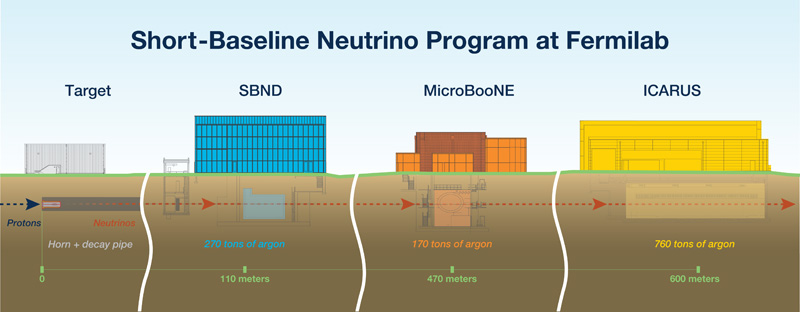
\includegraphics[width=1.0\textwidth]{SBN_program}
\caption[SBN_program]{
Graphic showing the three LArTPC detectors made up the Short-Baseline Neutrino program: SBND, MicroBooNE and Imaging Cosmic Rare Underground Signals (ICARUS).
Their respective masses and distances with to the target of the Booster Neutrino Beam are shown.
Fig. from \cite{SBNProgram}.
}
\label{fig:SBN_program}
\end{figure}


%Neutrino Cross Section
In additional, neutrino-nucleus interaction measurement is important in the physics program of SBND, which is critical element to understand neutrino oscillation \cite{}.
Being the nearest the detector to the beam presents the SBND experiment with a unique opportunity to observe the largest neutrino fluxes out of the three detector.
For 3 years of operation, SBND is expected to record 10 million neutrino events from $10 \times 10^{20}$ Proton-On-Target (POT) from the BNB.
SBND aims to be the world's largest statistics of neutrino-argon cross-section measurements.
More than 6 millions $\nu_{\mu}$ charged current (CC) events will be collected, reducing the statistics uncertainty well below the percent.
This measurement also allows for characterising the BNB neutrino flux, significantly improving neutrino flux modelling and hence, the associated uncertainty.
SBND is also expected to record 45,000 $\nu_{e}$ CC events, which will the largest statistics inclusive and exclusive measurement of this channel up-to-date.
These measurements will be extremely beneficial to the SBN physics program, as well as to DUNE physics program which will employ argon as the target material.

%BSM
Finally, a key part of the physics program of the SBND experiment is exploring new scenarios leading to physics BSM.
Specifically, being close up to a high intensity beam and therefore a large statistics allow for searches of very weakly coupled physics that is produced from the BNB. 
%HNL
Namely, Heavy Neutral Lepton, the main search of this thesis, can be produced by the BNB and then decay in-flight into SM observables for detection as detailed in Chapter \ref{}.
%Light Dark Matter
Another BSM candidate is light dark matter, which can be produced by neutral meson decay or proton bremsstrahlung in the BNB \cite{}.
These light dark matter particles are postulated by thermal relic models, and can reach mass sub-GeV scale.
They can scatter and decay inside the detector, producing electromagnetic showers without any hadronic activities.
%Dark neutrino
Furthermore, the dynamic mass mechanism of neutrino can lead to new physics in the dark sector. 
The dark neutrino model hypothesises a right-handed neutrinos can scatter with a nucleus to produce a dark gauge boson, and subsequently decay into a di-lepton pair \cite{}.
If discovered, this model can possibly explain the low energy excess anomalies seen by LSND by MiniBooNE.
These are a few of many BSM that can be probed at the SBND detector, that not yet mentioned such as new interactions, extra dimensions, violations of Lorentz and CPT symmetries and so on, adding to the very rich physics program of SBND.

%********************************** %First Section  **************************************
\section{The Booster Neutrino Beam}

%Describe rate
The SBND detector measures the neutrino flux coming from the Booster Neutrino Beam (BNB) \cite{}.
The full technical details of the BNB can be found in Ref. \cite{}.
Protons with 8 GeV kinetic energy are extracted from the Booster synchrotron at an average rate of 5 Hz (7 - 11 pulses in a row at 15 Hz).
Each spill delivers $5 \times 10^{12}$ protons over a total beam spill window of 1.6 $\mu$s.
A beam spill structure is made up 81 individual neutrino bucket, with a Gaussian sigma of 1.308 ns and period of 19 ns \cite{}.
The bucket beam structure can be resolved and utilised with nanosecond resolution, allowing for cosmics rejection outside of the bucket or searches for new physics \cite{}.
For example, the CRT system at SBND, with nanosecond timing resolution, was able to measure and resolve the beam bucket structure using a data set from 2007-2008 as shown in Fig. \ref{}.

%TODO: add 2007 - 2008 CRT plots

%hardware structure
The neutrino production in the BNB is illustrated in Fig. \ref{}.
Protons are injected into the Booster synchrotron and accelerated from 400 MeV to 8 GeV kinetic energy.
Their intensity is measured by two steroids whilst their positioning and timing are measured by beam position monitors and resistive wall monitor (RWM).
The RWM signal plays a key part in synchronising the DAQ of the SBND detector with respect to the beam and providing timing reference for high resolution analysis as discussed in Sec. \ref{}. 
Upon leaving the Booster, the proton beam is transported through focusing and defocusing quadrupole and dipole magnets, and eventually steered and focused onto the target of the BNB.
The target consists of a beryllium cylinder 71.1 cm long and 0.51 cm in radius. 
The choice of beryllium was motivated by replaceable ability in the case of radioactivity issues, as well as allowed for sufficient energy loss via air cooling system.
Protons interacting with the target produce secondary mesons and hadrons.
The target is placed inside a pulsed horn system which acts as a 170 kA electromagnet to focus the secondary particles.
The polarity of the horn can be chosen to focus positive (negative) hadrons for running in neutrino (antineutrino) mode.
A concrete collimator is located downstream of the horn assembly of size 214 cm long, 30 cm radius that grows to 35.5 cm from upstream to down stream end.
The collimator absorbs particles that would not contribute to the neutrino flux and hence, reduces radiation elsewhere in the beam line.
The focused particles then propagate down an air-filled cylindrical decay region, extending for 45 m and terminated by a steel and concrete absorber located 50 m from the upstream face of the target.
The short-lived secondary hadrons decay into tertiary neutrinos in this region, mean while long-lived muons are absorbed by the absorber to reduce the production of $\nu_{e}$.
The neutrinos then propagate through a dirt region before reach the SBND detector down stream.

%beam simulation
%Explain what meson is in the flux, what tuning is used, 
The beam is simulated using GEANT4 with different tunings for the composition of the secondary hadrons produced from $p + Be$.
The pion production is tuned to the HARP data set using Sanford-Wang fits \cite{}.
The positively charged kaon production is tuned to the global $K^{+}$ production data using Feynman scaling-based parametrisation \cite{}, and further constrained by SciBooNE's direct measurements of $K^{+}$ production from the BNB \cite{}. 
Other secondary hadrons such as protons, neutrons and $K^{-}$ produced is modelled using the MARS hadronic interactions \cite{}. 
Interactions cross sections of Beryllium nucleus with nucleons and pions are also used in flux predictions.   
The systematics uncertainties associated the BNB flux are calculated by a re-weighting process,
to be presented in Chapter \ref{}.

%TODO: add BNB secondary hadron profile plots
%TODO: add neutrino profile plots
%TODO: say something about kaon flux contributing to HNL here
As discussed in Sec. \ref{}, the main contributor to the HNL flux is the charged kaons $K^{+}$, which is made up of ?? in the BNB flux as shown in Fig. \ref{}.
The majority of HNL is produced from charged kaon decays with momentum peaking at 1 GeV.
Fig. \ref{} shows that the $K^{+}$ production cross section of the BNB has large uncertainties in this region, however, results from SciBooNE has demonstrated that the extrapolation of higher energy $K^{+}$ using Feynman scaling is valid \cite{}. 
Meanwhile, the simulation of the neutrino flux at the front face of SBND is shown in Fig. \ref{}, contributed by different types of neutrino.
Pion decay is the dominant production mechanism for both $\nu_{\mu}$ and $\bar{\nu}_{\mu}$, whereas muons produced from the pion decay is the primary source of $\nu_{e}$ at low energies.
Kaon production contributes significantly compared to that of pion.
A peak in the $\nu_{\mu}$ flux can be seen at half of the kaon mass (235.5 MeV) from kaon decay at rest \cite{}.



%********************************** %First Section  **************************************
\section{The Short-Baseline Near Detector}

The SBND detector is a LArTPC with an active volume of 112 tons and size 4 m (x-drift) $\times$ 4 m (y-height) $\times$ 5 m (z-length).
The detector is made of two TPCs sharing the same Cathode Plane Assembly (CPA) at the centre, each with a drift length of 2 m.
A complex Photon Detection System (PDS) is located behind each of the Anode Plane Assemblies (APAs) on the edege of the detector.
The PDS also includes a passive component made up of TPB-coated reflective foils installed at the CPA.
The entire detector is placed inside a membrane cryostat, and then is surrounded by seven planes of Cosmic Ray Tagger (CRT) to provide a full coverage for cosmic rejection.

\subsection{Time Projection Chamber}

%TODO: Add 3 figures TPC + Wireplanes + CE
%TODO: check number of wires

%APA
A single APA of SBND is a 4 m $\times$ 2.5 m steel frame supporting three wire planes: two induction planes, referred to as U and V, oriented at an angle $\pm 60^{\circ}$ to the vertical collection plane, referred to as Y, shown as green, blue and red in Fig. \ref{}.
Each wire plane consists of 150 $\mu$m diameter copper-beryllium wires with a wire pitch and a plane spacing of 3 mm.
The wires are tensioned to 7 N to prevent slackening when being cooled down at liquid argon temperature at 89 K\cite{}.
A biased voltage of -200 V, 0 V and 500 V is applied to the plane U, V and Y respectively to maintain charge transparency for the induction planes and collection efficiency for the collection plane.
A pair of coupled APA together form an APA plane as shown in Fig. {}, using jumper cables to connect across the 15 mm gap between the induction planes to form a single electronic channel.
In total, there are 5,632 wires in each TPC: 1,664 wires in the collection plane and 1,986 in each induction plane.

%CPA
The CPA plane consists of two steel frames, each made up of 8 windows, as shown in Fig. \ref{}.
Each window size 60 cm $\times$ 50 cm houses a fiberglass plate, laminated on both sides with non-conductive reflective foils with $> 99\%$ specular reflection in the visible range and evaporated with TPB.
The plate is covered by a wire mesh, which provide a biased voltage of -100 kV by a high voltage feed through donut from outside the cryostat. 

%Field Cage
The field cage comprises of a series of electrodes arranged perpendicular to the drift direction, gradually step up the voltage from -100 kV applied at the CPA to ground voltage in step of 3 kV increments.
This is to ensure a uniform electric field of 500 V/cm across the drift volume.


\subsection{Photon Detection System}

%\subsubsection{Photomultiplier Tubes}

%\subsubsection{X-ARAPUCAs}

%TODO: Add PDS box

%describe PMT, XARAPUCA and TPB
The design of SBND PDS, combining both active and passive optical component, is the most sophisticated system ever installed in a LArTPC.
The active detector integrates two different technologies: (1) a system made up of 120 PMTs and (2) a system of 192 X-ARAPUCA devices.
The PMTs are cryogenic 8"-diameter Hamamatsu R5912-MOD model \ref{}.
The X-ARAPUCAs serve as a R\&D ground for future experiments, and thus multiple variations in their components have been integrated for performance comparison.
A summary of the X-ARAPUCAs specification can be found in Ref. \cite{}.
Moreover, for a uniform light yield, the PDS in SBND also employs a passive component of TPB-coated foils located at the CPA plane as detailed in Sec. \ref{}.

In SBND, the PMT system is used to provide trigger conditions, and therefore serves as the primary light detection system.
The 120 PMTs are divided into 60 PMTs per optically-isolated TPC volume. 
In each TPC, 48 PMTs are TPB-coated and therefore sensitive to both direct and reflected light components, while the remaining 12 non-coated PMTs are only sensitive to reflected light.
This ratio of coated to uncoated (4:1) is chosen to maximise light collection efficiency whilst maintaining the ability to distinguish between the two light components.
This allows for improving the reconstruction of scintillation light discussed in Sec. \ref{}. 

%PDS Box
For installation purposes, the optical detectors are arranged into modular PDS boxes, as shown on the right of Fig. \ref{}.
Each box contains 5 PMTs, 4 coated and 1 uncoated, and 8 X-ARAPUCAs, 4 coated and 4 uncoated.
The PDS-boxes are installed in a 4 x 3 configuration behind each APA plane, adding to a total of 12 boxes per TPC volume as shown on the left of Fig. \ref{}.

\subsection{Cosmic Ray Taggers}

%TODO: Add CRT diagrams

SBND is a surface detector and therefore, and a Cosmic Ray Tagger (CRT) system is employed to reject background from cosmic rays.
A CRT strip is illustrated in Fig. \ref{}, made up of a scintillator strip connected connected to a pair of SiPMs via wavelength shifting optical fibres.
CRT strips are arranged perpendicular to each other to form a single CRT plane of size 7.5 m in height and 9 m in width.
The coincident hit from perpendicular strips allows for 2D reconstruction of the hit location.
The SiPMs are digitised and read out by the Front End Board (FEB) modules with nanosecond timing resolution (more detailed in Sec. \ref{}).

As depicted in Fig. \ref{}, SBND is completely surrounded by 7 CRT planes, 1 on each side and 2 on top of the detector. 
This allows for a comprehensive approach to reject cosmics background using a combination of geometrical information as well as high precision timing information. 
For example, tracks from the TPC can be matched to CRT hits to identify tracks occurring outside of the beam spill window.
Moreover, the top 2 planes form a telescopic array to tag vertical downward going cosmic rays.
 

\subsection{Trigger}

%TODO: add trigger diagram

Triggering is a vital component of the SBND detector due to close proximity to the BNB and therefore, a high rate of neutrino events.
The hardware trigger at SBND is issued by the Penn Trigger Board (PTB), which receives inputs from the beam system and two detection systems with high timing resolution, the PMTs and CRTs.
The PTB applies programmable trigger logic on the inputs to form triggers.
There are three main types of triggers for different purposes: (1) beam trigger to acquire physics data, (2) off-beam trigger for cosmic background estimation and (3) calibration trigger.

The beam system inform the PTB of the status of the BNB beam, whether the beam arrives at the detector hall.
The PMTs provide information regarding the energy deposited inside the detector, based on the numbers of PMT pairs above a given threshold. 
The main beam trigger will require the PMT multiplicity to be in coincidence with the beam window.
Meanwhile for background estimation purpose, anti-coincidence logic can be applied to estimate the rate of cosmics.
Meanwhile, the CRT system provide versatile information regarding the topology of a cosmic tracks.
Calibration trigger will use the CRTs in coincidence with the PMTs to select cosmic tracks of specific topologies, for example, anode-to-cathode-crossing cosmics can be used for electron lifetime measurement.

Once a trigger is formed, the PTB send the signals to subsequent readout subsystems to acquire the event.
An event contains two types of trigger signals: a single Event trigger and multiple Flash triggers.
The Event trigger is issued to the TPC readout subsystem to acquire waveforms from the wire planes, whilst Flash triggers are issued to the PDS subsystems to acquire waveforms from the PDS.
Th details will of the data acquisition employing these two types of signal is discussed in the following section.


\subsection{Data Acquisition}

%\section{Overview of the Data Acquisition System}
\label{sec4Overview}

%short description of daq
Data Acquisition (DAQ) is responsible for transporting data from subsystem hardware to event builder machines.
During real-time data flow, the DAQ must have the capability for event building by assembling data from each subsystem hardware into a cohesive physics event. 
Additionally, the DAQ must be able to apply complex software metrics to filter events for various data streams and data monitoring purposes.

%describe daq component
At SBND, the DAQ comprises six hardware subsystems illustrated in Fig. \ref{fig:daqOverview}.
Among these, four are the detection subsystems: the Time Projection Chamber (TPC), Photomultiplier Tubes (PMTs), X-ARAPUCAs, and Cosmic Ray Taggers (CRTs).
Each detection subsystem incorporates specialized hardware components for digitizing and reading out the physical signals. 
Moreover, two other subsystems are the Penn Trigger Board (PTB) \cite{ptb_gvs} and the SPEC-TDC. 
The PTB, as a hardware board within the SBND trigger system, is responsible to provide triggering signals to each detection subsystem independently.
The SPEC-TDC is a specialised timing mezzanine module designed specifically for timestamping purposes.
%TODO:FIX!
%Further details about its functionality are outlined in section \ref{subsec42TimeRef}.

\begin{figure}[htbp!] 
\centering    
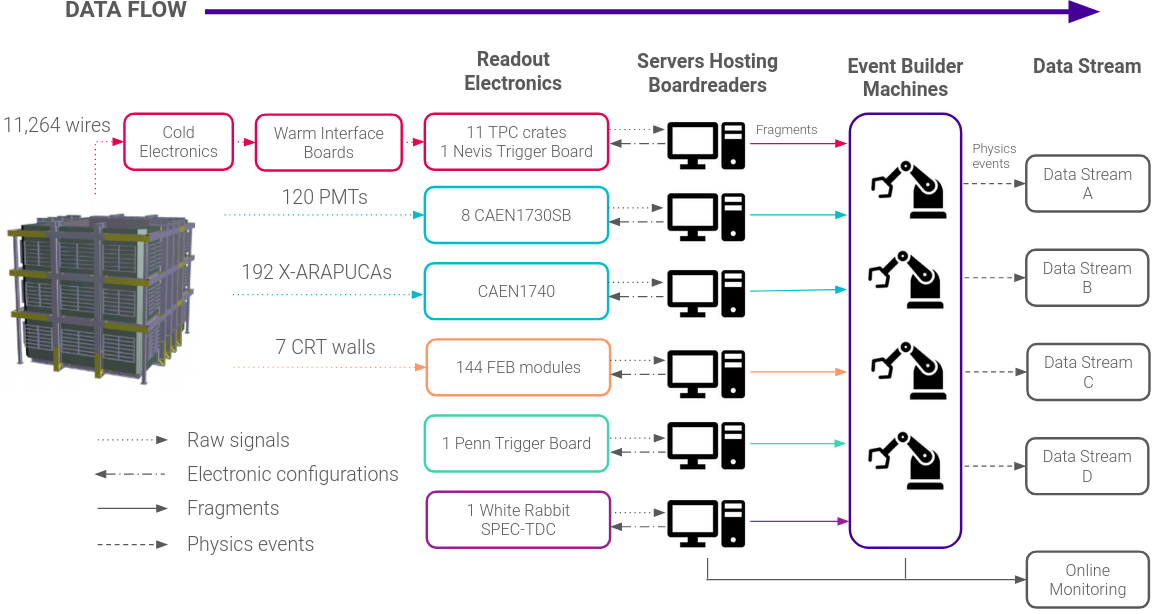
\includegraphics[width=1.0\textwidth]{DAQ_Overview}
\caption[DAQOverview]{
The DAQ system at SBND consists of six subsystems, with four dedicated to detection subsystem readouts for the TPC, CRTs, PMTs and X-ARAPUCAs, while the remaining two facilitate triggering and timing functionalities.
Each hardware component is accompanied by a corresponding software boardreader, serving as a communication bridge between the hardware and the event builder machines.
The event builders assemble a physics events and send it to different data streams for storage.
}
\label{fig:daqOverview}
\end{figure}

The DAQ software framework is provided by the \textit{artdaq Toolkit}, developed by the Real-Time Systems Engineering Department of Fermilab's Scientific Computing Division \cite{artdaq_note}.
The software acts as the backbone of the communication between the hardware components and the event builder machines.
The following section provides an overview of the DAQ workflow at SBND as illustrated in Fig. \ref{fig:daqOverview}, describing how signals are acquired from the detection hardware and subsequently digitized by boardreaders and assembled into a physics event.

%describe boardreader fragment
Within the \textit{artdaq} framework, each discrete hardware readout component has a corresponding software, known as a boardreader, facilitating communication between the readout electronics and the event builder machines.
The boardreader can send configurations directly to the hardware in one direction and retrieves data from the hardware in the opposite direction.
The data is packaged into a digitized format called a fragment as depicted in Fig. \ref{fig:fragmentDiagram}. 
The fragment class includes a header containing experiment-specific information essential for event building, an optional metadata, and a data payload storing the hardware-defined data.
A fragment is generated by the boardreader when its corresponding hardware readout receives a trigger.
The timestamp of the trigger arrival is encoded in the fragment header, which is known as the fragment timestamp.
This timestamp is the crucial value in the event building process.

\begin{figure}[htbp!] 
\centering    
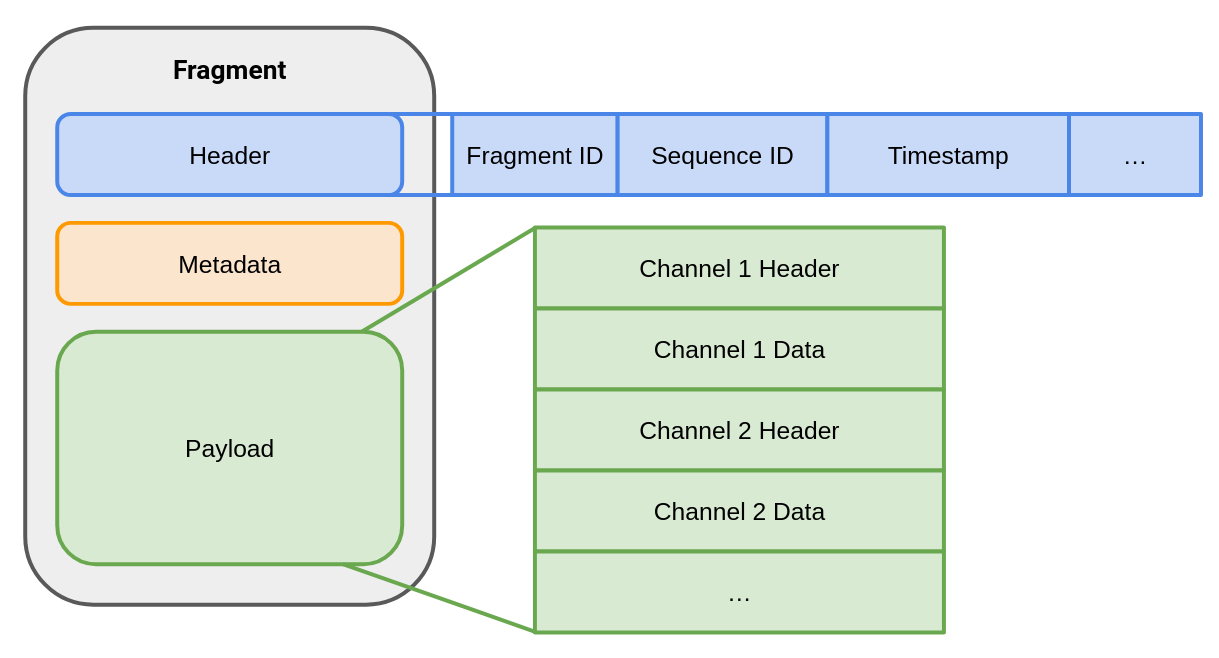
\includegraphics[width=0.6\textwidth]{Fragment_Diagram}
\caption[FragmentDiagram]{This diagram illustrates the fragment class defined by the \textit{artdaq Toolkit}. The header contains information needed for event building, of which the key information is the fragment timestamp. Optionally, the metadata structure contains hardware configurations. The payload is designated for storing data from the hardware readout, of which the data structure is pre-defined by the hardware. }
\label{fig:fragmentDiagram}
\end{figure}

%what is push/pull
Once fragments are generated, boardreaders can send them to the event builders in either one of the two configurations: push or pull. 
When operating in the push configuration, the boardreader actively sends fragments continuously at the rate at which the fragments are generated.
The sequence ID of the fragments determines the sequence ID of the built event, ensuring  that every fragment is built as a single event.
With each fragment sent, the push boardreader also creates a request message, which is multicast to all other boardreaders currently in pull mode.
This request message contains the timestamp of the push fragment. 

In contrast to the push configuration, the boardreader in the pull configuration stores the fragments in its buffer as the fragments are being generated.
These fragments are sent to the event builders only upon receiving a request message.
To determine which fragments to send, the boardreader has a configurable parameter called pull window, which specifies a time window relative to the timestamp of the request message.
The pull boardreader checks its buffer and selects the fragments with timestamps falling within this defined time window.
The selected fragments that meet the timestamp requirement are then dispatched to the event builders.
Subsequently, the event builder machines compile this set of fragments, together with one single fragment from the push boardreader that initially generated the request message, into a single event.
The sequence ID of the resulting event is determined by the push fragment.

\begin{figure}[htbp!] 
\centering    
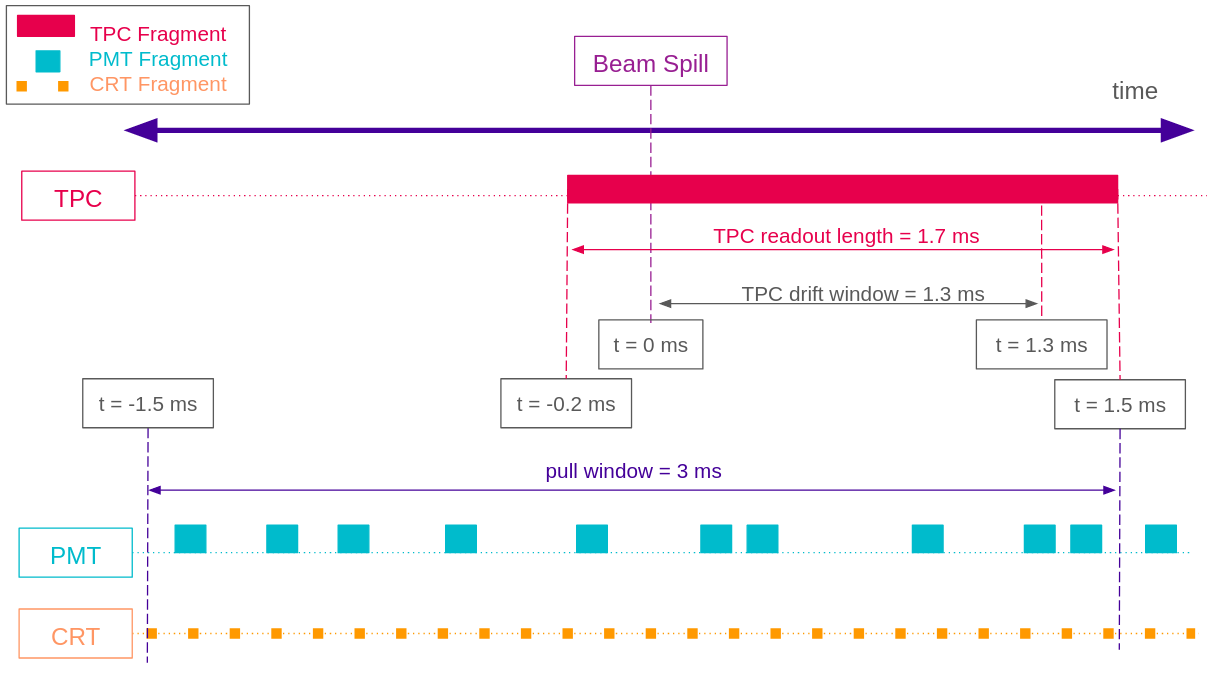
\includegraphics[width=1.0\textwidth]{SBND_Event_Structure}
\caption[SBNDEventStructure]{
This cartoon depicts a physics event structure at SBND, where the time axis is centred at 0 for when the beam spill begins. 
The event contains TPC fragments of readout length 1.7 ms to fully cover the drift window of an ionised electron from cathode to anode. 
The fragments generated by the PMTs and CRTs readouts are included 1.5 ms before and after the beam spill starts. 
The time asymmetry of the event structure is due to scintillation photon signals are produced and digitised much faster compared to electron signals.}
\label{fig:SBNDEventStructure}
\end{figure}

%describe an event structure
A physics event during at beam spill at SBND is built based on the structure shown in Fig. \ref{fig:SBNDEventStructure}, using the fragments from the three detection systems: TPC, PMTs and CRTs.
\footnote{13th November 2023: The DAQ hardware and software for the X-ARAPUCAs is under development and therefore, not be included in this thesis. }
Within this structure, there is only one push boardreader that increments the event sequence ID counter whilst the remaining boardreaders run in pull configuration.
The push boardreader is called the Nevis Trigger Board (NTB), which is a component of the hardware complex to readout the TPC data. 
The PTB sends a single Event trigger to the NTB that coincides with the start of the BNB beam spill if it determines a neutrino event occurs.
This generates a TPC fragment has a readout length of 1.7 ms, that fully covers the TPC drift length of 1.3 ms, and includes a padding of 0.2 ms before and after the drift.
The Event trigger timestamp is encoded in the NTB fragment header.

Meanwhile, the boardreaders for the PMTs and CRTs are in pull mode.
The PTB sends multiple Flash triggers to the PMTs readouts throughout the beam spill and CRTs readouts are self-triggered independently.
The fragment readout lengths from the PMTs and CRTs readouts are much shorter compared to TPC fragments, in the order of $\mu$s and ns respectively.
The pull window is defined to be 3 ms centred on the timestamp of the NTB fragment, to include PMTs and CRTs fragments generated 1.5 ms before and after the beam spill starts.
The event builders then package all the these fragments together to form a physics event.

%event asymmetry
The event structure has an asymmetry in time due to the physics characteristics of photon signals, detected by the CRTs and PMTs, and electron signals, detected by the TPC wires.
Photon signals are much faster than electron signals.
A photon produced in CRT scintillator strip takes approximate 5 ns to travel from the far end of the strip until the readouts.
A photon produced in the TPC takes maximum 15 ns to arrive at the PMTs from the scintillation location.
An ionised electron produced at the same time in the TPC takes 1.3 ms to fully drift from the cathode to the anode.
Therefore, scintillation photon signals produced during the beam spill need be digitized and readout much earlier compared to the electron signals.

%describe a data stream
After the event builder machines complete building a physics event, the resulting event can be filtered and sent to various locations for serving different downstream analysis purposes. 
This process is commonly referred to as data streaming.
The \textit{artdaq Toolkit} provides options to add customisable filtering steps in real-time, such that the event builders can apply complex software metrics based on the fragment contents of an event.
Once an event passes the filter, the event builders send it to a location defined by the filter.
If an event does not pass the filters, it will be dropped in real-time.

\begin{figure}[htbp!] 
\centering    
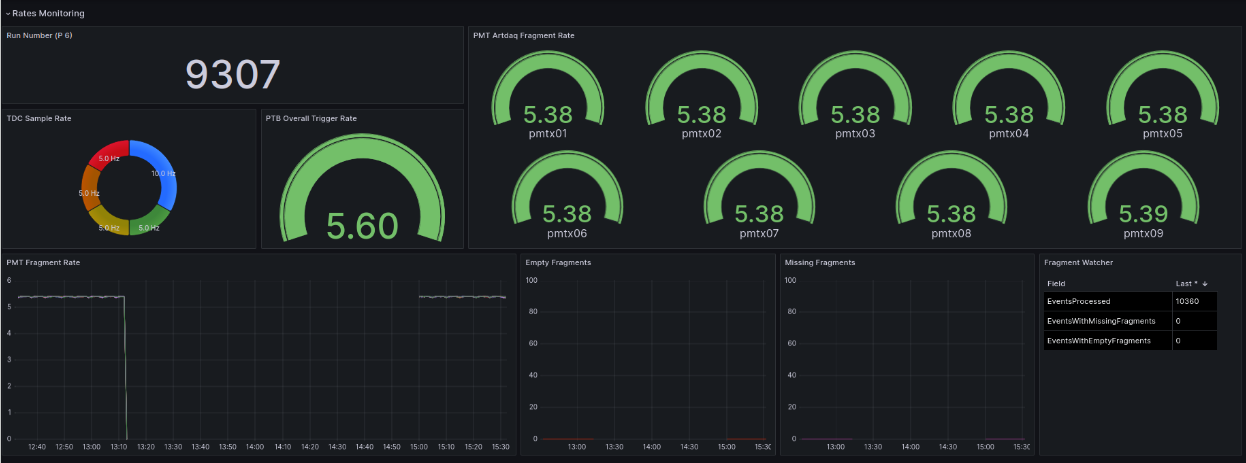
\includegraphics[width=1.0\textwidth]{Grafana}
\caption[Grafana]{
This screenshot displays a section of the Grafana monitoring website for the boardreaders of the PMT DAQ.
Some key information to quickly evaluate the status of the PMT boardreaders are shown.
For example, the fragment generation rate is expected be consistent with the trigger rate sent by the PTB whilst the empty fragment rate and the missing fragment rate stay flat at zero.
}
\label{fig:Grafana}
 \end{figure}

\begin{figure}[htbp!] 
\centering    
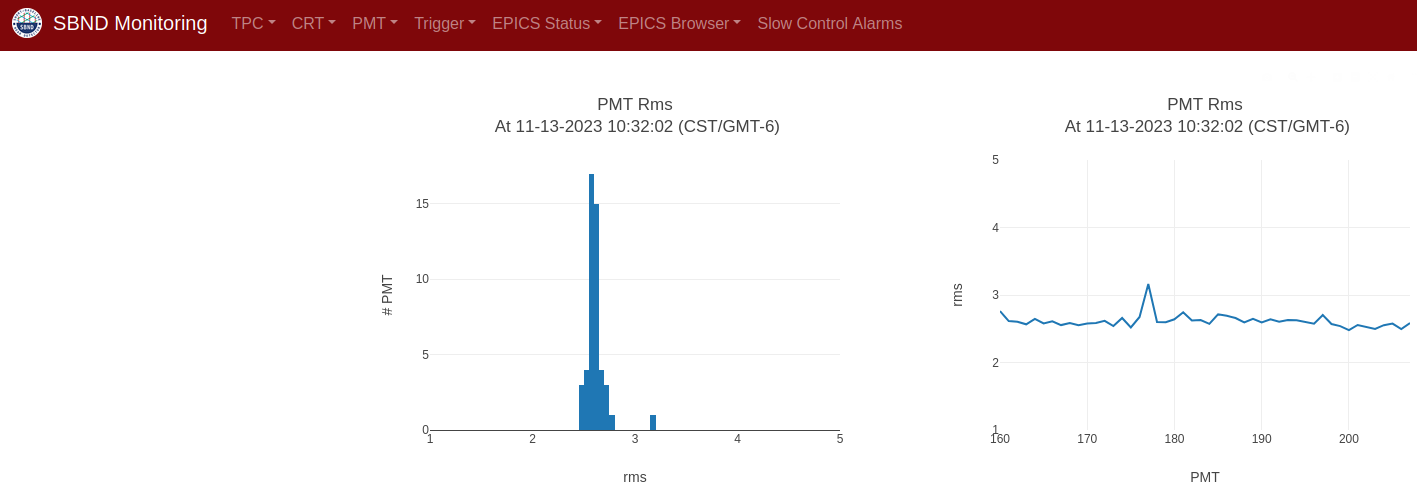
\includegraphics[width=1.0\textwidth]{Minargon}
\caption[Minargon]{
This screenshot displays a section of the Minargon monitoring website to evaluate the quality of data acquired by the PMT DAQ.
For example, a metric shown here is the waveform baseline RMS, plotted as a histogram (left) and plotted with respect to the fragment timestamp (right).
This metric provides monitoring of the baseline equalisation and stability over time.
}
\label{fig:Minargon}
\end{figure}

%data monitoring?
The \textit{artdaq Toolkit} also has a built-in process the bridges the event builder machines and online monitoring platforms.
Whilst running in real-time, fragments from boardreaders and physics events can be sent to the platforms for different monitoring purposes.
SBND currently employs two online platforms that monitors the health of the DAQ: Grafana and Minargon.
Grafana, as displayed in Fig. \ref{fig:Grafana}, provides real-time monitoring of the status of processes being run by boardreaders and event builders. 
Grafana monitoring also extends to include some status of the respective hardware component for each boardreader.
Minargon, as displayed in Fig. \ref{fig:Minargon}, provides real-time the data quality monitoring. 
This online monitoring process applies simple reconstruction and event display in order to quantitatively verify the physics characteristics of an event. 
The author has worked extensively on developing the monitoring processes for the DAQ of the PMTs on both Grafana and Minargon monitoring platforms during her PhD course. 

\subsubsection{TPC Cold Electronics and DAQ}

%Cold Electronic

\subsubsection{PDS DAQ}

\subsubsection{CRT DAQ}

%********************************** %First Section  **************************************
\section{Concluding Remarks}
